\documentclass[letterpaper, 11pt]{extarticle}
% \usepackage{charter}
% \usepackage{fontspec}
% \setmonofont{Fira Code}[
%   Contextuals=Alternate  % Activate the calt feature
% ]

% ==================================================

% document parameters
% \usepackage[spanish, mexico, es-lcroman]{babel}
\usepackage[english]{babel}
\usepackage[margin = 0.5in]{geometry}

% ==================================================

% Packages for math
\usepackage{mathrsfs}
\usepackage{amsfonts}
\usepackage{amsmath}
\usepackage{amsthm}
\usepackage{amssymb}
\usepackage{physics}
\usepackage{dsfont}
\usepackage{esint}
\usepackage{mathtools}

% ==================================================

% Packages for writing
\usepackage{enumerate}
\usepackage[shortlabels]{enumitem}
\usepackage{framed}
\usepackage{csquotes}
% \usepackage{booktabs}

% ==================================================

% Miscellaneous packages
\usepackage{float}
\usepackage{tabularx}
\usepackage{xcolor}
\usepackage{multicol}
\usepackage{subcaption}
\usepackage{caption}

\captionsetup{format = hang, margin = 10pt, font = small, labelfont = bf}
% \usepackage{todonotes} % todo margins/inline
\usepackage{changepage} % indentation

% Citation
\usepackage[round, authoryear]{natbib}

% Hyperlinks setup
\usepackage{hyperref}
\definecolor{primary}{HTML}{cb0062}
% \definecolor{links}{rgb}{0.36,0.54,0.66}
\hypersetup{
   colorlinks = true,
    linkcolor = primary,
     urlcolor = primary,
    citecolor = blue,
    filecolor = blue,
    pdfauthor = {Author},
     pdftitle = {Title},
   pdfsubject = {subject},
  pdfkeywords = {one, two},
  pdfproducer = {LaTeX},
   pdfcreator = {pdfLaTeX},
   }
\usepackage{cleveref}
\usepackage{titlesec}
\usepackage[many]{tcolorbox}

% \usepackage{fontspec}

% Adjust spacing after the chapter title
\titlespacing*{\chapter}{0cm}{-2.0cm}{0.50cm}
\titlespacing*{\section}{0cm}{0.50cm}{0.25cm}

% Indent 
\setlength{\parindent}{0pt}
\setlength{\parskip}{1ex}

% --- Theorems, lemma, corollary, postulate, definition ---
% \numberwithin{equation}{section}


\newtcbtheorem[]{problem}{Problem}%
    {enhanced,
    colback = black!5,
    colbacktitle = black!5,
    coltitle = black,
    boxrule = 0pt,
    frame hidden,
    borderline west = {0.5mm}{0.0mm}{black},
    fonttitle = \bfseries\sffamily,
    breakable,
    before skip = 3ex,
    after skip = 3ex
    }{problem}


\newtcbtheorem[]{solution}{Solution}%
    {enhanced,
    colback = green!5, %white,
    colbacktitle = green!5,
    coltitle = black,
    boxrule = 0pt,
    frame hidden,
    borderline west = {0.5mm}{0.0mm}{black},
    fonttitle = \bfseries\sffamily,
    breakable,
    before skip = 3ex,
    after skip = 3ex
}{problem}

\tcbuselibrary{skins, breakable}

% --- You can define your own color box. Just copy the previous \newtcbtheorm definition and use the colors of yout liking and the title you want to use.

\begin{document}

\begin{Large}
    \textsf{\textbf{EE 150 [Winter 2024]}}
    
    \textsf{Problem Set 1}
\end{Large}

\vspace{1ex}

\begin{tabbing}
    \hspace{10em} \= \kill
    \textsf{\textbf{Due:}} \> \textsf{01/22/25 at 9:00 p.m.} \\
    \textsf{\textbf{Submit:}} \> \textsf{on \href{https://gradescope.com}{gradescope}} \\
    \textsf{\textbf{Collaborators:}} \> \textsf{None} \\
    \textsf{\textbf{Teaching Assistants:}} \> \href{https://armeet.ca}{Armeet Singh Jatyani} \& \href{https://github.com/PipeCruz}{Felipe Cruz}
\end{tabbing}


\vspace{2ex}

Welcome to EE 150! Collaboration is allowed, just list the names of the people
you collaborated in the header. If you choose to use Latex to type your
submission, we recommend filling in this template.

To prepare your code submission, run \verb|zip_assignment.py| from the root of
the project folder and upload that zip to the code part of the assignment on
gradescope.

If you have any other questions, come to office hours or ask us on Piazza for a
quick response.


\begin{problem}{Convolutional Neural Networks \hfill [40 pts]}{prob:cnns}
\label{prob:cnns}

\begin{adjustwidth}{2em}{2em}
    
    \textbf{(a)} \textbf{Write a convolution algorithm from scratch} \hfill (10 pts)
    \begin{adjustwidth}{2em}{2em}
    
    i) Implement the \texttt{Conv2d} class in \texttt{conv.py}. \\
    
    ii) Implement the \texttt{FasterConv2d} class in \texttt{conv.py}. Ensure all tests in $\texttt{conv\_tests}$ pass.\\
    
    iii) Run $\texttt{benchmark\_conv2d.py}$ to compare your implementations to the PyTorch Implementation. For a batch of 16 $28 \times 28$ images, how many times faster was your faster implementation compared to your initial implementation and the PyTorch implementation compared to your faster implementation?
    \\
    
    iv) Give a reason for why the PyTorch implementation is faster. \\
    \end{adjustwidth} 
    \vspace{5px}

    \textbf{(b)} \textbf{Implement and train a CNN to classify MNIST} \hfill (5 pts)
    \begin{adjustwidth}{2em}{2em}
    
    i) Implement the \texttt{CNN} class in \texttt{cnn.py}. \\
    
    ii) Complete the \texttt{TODO}s in \texttt{train\_test.py} that are needed to train the CNN. Then, run \texttt{train\_mnist.py} to achieve at least $96\%$ test accuracy after 5 training epochs. After training, take a look at the $\texttt{results/}$ folder to find results, plots, and the saved model. Attach your accuracy and loss plots here and report your test accuracy.

    \\

    \end{adjustwidth} 
    \vspace{5px}

    \textbf{(c)} \textbf{Manually picking filters} \hfill (5 pts)
    \begin{adjustwidth}{2em}{2em}
    Copy any necessary code from your \texttt{CNN} class to the \texttt{ManualCNN} class. Now, instead of letting the convolutional layer learn 4 filters, you will set the 4 filters manually based on what filters might result in features useful for distinguishing numbers. Initialize $\texttt{self.conv.weight.data}$ manually and note that we set $\texttt{self.conv.weight.requires\_grad}$ to $\texttt{False}$ so the filters remain fixed during training (only the fully-connected layer will train). Your goal is to achieve at least 94\% test accuracy. Take a look at the $\texttt{ArgumentParser}$ in $\texttt{train\_mnist.py}$ to determine how to train the $\texttt{ManualCNN}$. Attach your accuracy and loss plots here and report your test accuracy. Once you are satisfied with the performance of your filters, run $\texttt{visualize\_filters.py}$ to visualize your chosen filters' effects on MNIST digits. Note that it requires the path to your saved $\texttt{ManualCNN}$ model. Attach the visualization here.\\
    \end{adjustwidth}
    \vspace{5px}
    \textbf{(d)} \textbf{Transfer Learning using AlexNet on PCAM image dataset} \hfill (5 pts)
    \begin{adjustwidth}{2em}{2em}
        i) What is AlexNet and why is it such a big deal? (1 sentence) \\

        ii) Make a copy of \href{https://colab.research.google.com/drive/1HnRFDWtVqBgMh-9sSF1WnHwGJQ5bvLXF?usp=sharing}{this notebook}, complete it, and provide a link to your colab notebook that is shareable. Make one observation of the loss/accuracy plots at the end and give a reason for it.  \\
    \end{adjustwidth}
    \textbf{(e)} \textbf{Why skip connections prevent vanishing gradients} \hfill (10 pts)
    \begin{adjustwidth}{2em}{2em}

    Consider an $L$-layer neural network with each layer having a width of 1. Let $h^{(0)}$ be the input of the network and for $l = 1, \dots, L$, define
    $$h^{(l)} = \sigma(w^{(l)}h^{(l - 1)} + b^{(l)})$$
    where $h^{(L)} = \hat{y}$ is the output of the network.

    i) Write an expression for $\frac{\partial \mathcal{L}}{\partial w^{(1)}}$ incorporating terms of the form $\frac{\partial h^{(l)}}{\partial h^{(l-1)}}$. \\

    ii) Write an expression for $\frac{\partial h^{(l)}}{ \partial h^{(l-1)}}$. Treat $\sigma$ as an arbitrary activation function. Then, compute this expression for $h^{(l - 1)} = 0.1, w^{(l)} = 0.1, b^{(l)} = 0$ and $\sigma(z) = \text{ReLU}(z)$. \\

    iii) If $\left|\frac{\partial h^{(l)}}{ \partial h^{(l-1)}}\right| < 1$, what happens to $\frac{\partial \mathcal{L}}{ \partial w^{(1)}}$ for large $L$? Why does this harm training? What about if $\left|\frac{\partial h^{(l)}}{ \partial h^{(l-1)}}\right| > 1$? \\
    
    iv) Let's say we add skip connections to our neural network. This means that
    
    $$h^{(l)} = \sigma(w^{(l)}h^{(l - 1)} + b^{(l)}) + h^{(l - 1)}$$
    
    Write an expression for $\frac{\partial h^{(l)}}{ \partial h^{(l-1)}}$ and explain how the skip connection alleviates the vanishing gradient problem. \\
    
    \end{adjustwidth}

    
    
    \textbf{(f)} \textbf{Visualize loss landscape of ResNet} \hfill (5 pts)
    \begin{adjustwidth}{2em}{2em}
        \href{https://arxiv.org/abs/1512.03385}{ResNet} is a CNN architecture that takes advantage of residual connections (skip connections) to train very deep networks reliably. It is the most widely used CNN architecture today. Visit this \href{http://www.telesens.co/loss-landscape-viz/viewer.html}{link} to view some visualizations of the loss landscape for various ResNets with and without skip connections. ``No short'' means without skip connections. \\
        

        i) Explain the difference between the loss landscapes of ResNet20 (No short) and ResNet56 (No short). (1 -- 2 sentences) \\

        ii) Compare the loss landscapes of ResNet56 (No short) to ResNet56 (short). In terms of minimizing loss, why is the ResNet56 (short) loss landscape preferable? (1 -- 2 sentences)
        
    \end{adjustwidth}
\end{adjustwidth}

\end{problem}

\begin{solution*}{}{}
Student solution here.
\end{solution*}
\begin{problem}{Autograd from Scratch \hfill {[20 pts]}}{prob:autograd}
\label{prob:autograd}

In this problem, you will implement your very own \textit{scalar autograd}
(differentiation) library. If you're scared, don't be! You'll be writing just
100-150 lines of Python code in 2 files. This problem aims to introduce you to
automatic differentiation and backpropagation by demonstrating how they work at
the scalar (single number) level. More advanced libraries like PyTorch, JAX, and
TensorFlow/Keras extend these concepts to the tensor/matrix/vector levels for
automatic differentiation. This assignment is inspired and adapted from Andrej
Karpathy's \verb|micrograd| \cite{Andrej2024karpathy}.

\vspace{10px}
\textbf{Setup}

Download the assignment \verb|.zip| from Gradescope and extract it somewhere on
your computer. Follow the project setup in \verb|SETUP.md|. It'll guide you on
how to install \verb|graphviz| and \verb|uv|, which we'll be using to manage
your python environment. We've also made a setup video guide
\href{https://youtu.be/9R_9iv-Y4Ts}{here}.

\vspace{10px}
\textbf{Automatic Differentiation}

Say we have an expression $y = ax + b$. We know that $\frac{\partial y}{\partial
x} = a$ or $\frac{\partial{y}}{\partial a} = x$ or $\frac{\partial y}{\partial
b} = 1$, but how do we calculate these partial derivatives automatically? What
about far more complex expressions with nested structures?\\

The idea is to wrap constants and variables (to us they are all unit values)
like $a, b, x$ in a \verb|Value| object/class (which you will implement), to
exploit the modularity of both the "forward" and "backward" computation logic.
So $3.14 \rightarrow \verb|Value(3.14)|$. Then, we can construct complex
expressions with these unit \verb|Value|'s as building blocks. Under the hood,
we will automatically construct a computation graph (DAG) as visualized in
\cref{fig:handbackprop}. \verb|Value| objects have methods that allow them to
interact with other \verb|Value|'s. For instance, you will implement functions
for adding, subtracting, multiplying, and dividing any two \verb|Value| objects
as well as special transformations called \textit{non-linearities} (ReLU,
Sigmoid, tanh). For example, $\verb|Value(3.14).sigmoid()| = \sigma(3.14) =
\frac{1}{1 + e^{-3.14}}$. Finally, you will implement the backbone of the
autograd engine, the \verb|backward()| method, which relies on the computation
graph we constructed when piecing together values.\\

\vspace{10px}
\textbf{Gradient Back-propagation}

To find the gradient of the loss function $L$ with respect to a parameter $w$,
we use the chain rule. $w_{next}$ is the node right after the current parameter
$w$, so in \cref{fig:handbackprop} if $w=w_1$ then $w_{next}=s$.

\[
\frac{\partial L}{\partial w} = 
\underbrace{\frac{\partial L}{\partial w_{next}}}_{\text{Gradient of next value.}} \cdot 
\underbrace{\frac{\partial w_{next}}{\partial w}}_{\text{Local gradient}}
\]


Start by reading \verb|grad/autograd.py|. Understand the \verb|__init__|,
\verb|__repr__|, \verb|parse|, and \verb|__add__| functions in the \verb|Value|
class.\\

Implement the following functions to enable \texttt{Value} operations. We've
done \verb|__add__| and \verb|__radd__| for you already, so read through those
first. If you don't follow a similar order/structure, we cannot guarantee that
your tests will pass. To understand what \verb|__radd__| does, read the first
response to
\href{https://www.reddit.com/r/learnpython/comments/3cvgpi/can_someone_explain_radd_to_me_in_simple_terms_i/}{this
thread}. Run tests with \verb|uv run tests.py| or \verb|python tests.py| from
the root directory after you implement each function! These functions are
methods of the \verb|Value| class, so \verb|self| refers to the current object,
and \verb|other| refers to the other object. For example, Python maps
\verb|val_a + val_b| to the \verb|__add__| function with \verb|self=val_a| and
\verb|other=val_b|.\\

\textbf{CAREFUL:} When updating \verb|self.grad| in these parts, use
\verb|self.grad +=| instead of \verb|self.grad =| because the same \verb|Value|
can be used twice in an expression, so we should be accumulating gradients, not
overwriting what's already in a \verb|Value|'s \verb|self.grad| field.

\begin{adjustwidth}{2em}{2em}
    \textbf{(a)} \verb|__mul__| (self * other) \hfill (2 pts)\\
    \textbf{(b)} \verb|__sub__| (self - other) \hfill (2 pts)\\
    \begin{adjustwidth}{2em}{2em}
    hint: addition and negation\\
    \verb|__neg__| is already implemented for you\\
    \end{adjustwidth}
    \textbf{(c)} \verb|__pow__| (self ** other) \hfill (2 pts)\\
    \textbf{(d)} \verb|__truediv__| (self / other) hint: multiplication and
    power \hfill (2 pts)\\
\end{adjustwidth}

Now you'll implement some non-linear transformations, often called
\textit{nonlinearities}. Specifically, you'll implement the ReLU, sigmoid, and
tanh transformations. We use these non-linear transformations later when
building neural networks. Where possible, try to reuse code by calling the
earlier functions. Some functions and derivatives can be represented in terms of
themselves, or other previously handled cases. You may use the \verb|math|
library to compute values of tanh(x) or exp(x).

\vspace{10px}
\begin{adjustwidth}{2em}{2em}
    \textbf{(e)} \verb|f_relu| \hfill (2 pts)\\
    \textbf{(f)} \verb|f_sigmoid| \hfill (2 pts) \\
    \textbf{(g)} \verb|f_tanh| \hfill (2 pts)\\
\end{adjustwidth}
\vspace{10px}


To the final part of this problem! Implement the following\ldots

\vspace{10px}
\begin{adjustwidth}{2em}{2em}
\textbf{(h)} \verb|backward| \hfill (3 pts)\\
\textbf{(i)} {Compare with hand-backpropagation} \hfill (3 pts)\\

\begin{adjustwidth}{2em}{2em}
You will complete a few lines in \verb|examples/ex_2i_backprop.py|. In
problem 1, we did backpropagation by hand, for the expression $L = (w_1 +
w_2) \cdot w_3$. Recreate this same expression from \cref{fig:handbackprop}
and complete all TODOs. Run the script to generate
\verb|figs/ex_backprop_before.png| and \verb|figs/ex_backprop_after.png|.
Include both in your submission and comment on whether the calculated
gradients, updated parameters $w_1,w_2,w_3$, and new result value $L$ match
with your previous results in Problem 1.\\
\end{adjustwidth}

\vspace{10px}
You've successfully implemented an autograd engine that is capable of minimizing
any expression that can be composed by your \verb|Value| class (which supports
basic operations, in addition to three non-linearities). Notice that any loss
function $L$ that can be defined in terms of \verb|Value|'s  can be minimized
with our autograd library.\\
    
\end{adjustwidth}
\vspace{10px}
\end{problem}


\begin{solution*}{}{}
\begin{center}

\includegraphics[width=\textwidth]{../figs/ex_backprop_before.png}

\includegraphics[width=\textwidth]{../figs/ex_backprop_after.png}
\end{center}
\end{solution*}


\begin{problem}{Transformers \hfill [20 pts]}{prob:rnns}
\label{prob:rnns}

\begin{adjustwidth}{2em}{2em}
    
    \textbf{(a) Attention } \hfill (10 pts) 
    
    \begin{adjustwidth}{2em}{2em}
    i) Write down the scaled dot-product self-attention function $\text{Attention}(x)$ in terms of $x, W_q, W_k, W_v$, and $d_k$. What are the shapes of $x, W_q, W_k, W_v$ in terms of sequence length $T$, embedding dimension $D$, key dimension $d_k$, and value dimension $d_v$? For simplicity, we are not considering the batch dimension because in implementation this function is applied to every sequence in the batch the same way. You can use the function $\text{softmax}(z)$ without defining it. What is the shape of the output of $\text{Attention}(x)$?
    \\

    ii) The gradient of the softmax function is very small for inputs of large magnitude. Assume that $Q = xW_q$ and $K = xW_k$ are random variables sampled from a multivariate standard normal and $T = 1$. What is the distribution of the input to the softmax function if we don't scale the input by $1/\sqrt{d_k}$? Why does scaling by $1/\sqrt{d_k}$ alleviate the aforementioned issue? Hint: Write out the dot product and apply the Central Limit Theorem.
    \\

    iii) Write down how to compute multi-head self attention in terms of $x, W_o,$ the sequences of matrices $\{W_k^i\}_{i = 1}^h$, $\{W_q^i\}_{i = 1}^h$, $\{W_v^i\}_{i = 1}^h$, $d_v$, and $d_k$, where $h$ is the number of heads. Again, you can use $\text{softmax}(z)$ without defining it. What are the shapes of $W_k^i$, $W_q^i $, $W_v^i$, and $W_o$? Assume that the outputs have dimension $D$.
\\

    iv) Implement the \texttt{SelfAttention} class in \texttt{attention.py}. Implement the \texttt{MultiHeadAttention} class as well. Ensure all the \texttt{attention\_tests} pass. 

    \end{adjustwidth} 
    \vspace{5px}

    
    \textbf{(b)} \textbf{Train Transformer on IMDB Reviews to classify sentiment} \hfill (5 pts)
    \begin{adjustwidth}{2em}{2em}

    Implement the \texttt{TODO}s in \texttt{transformer.py}. Train the Transformer using \texttt{train\_imbd.py} for 5 epochs, a minimum sequence length of 0 and a maximum sequence length of 200. Then train the Transformer for 5 epochs, on a minimum sequence length of 200 and a maximum sequence length of 400. Attach your accuracy and loss plots here for both models and report test accuracies.
        \end{adjustwidth} 

        \vspace{5px}

    \textbf{(c)} \textbf{Compare Sequence Models} \hfill (2.5 pts)
    \begin{adjustwidth}{2em}{2em}
        Fill in the following table with test accuracies of all the models. Note that architecture hyperparameters were already adjusted for you so that each model has the same number of parameters, making this a fair comparison. What do you notice? (1 -- 2 sentences)

        \begin{center}
            \begin{tabular}{|l|c|c|}
            \hline
            \textbf{Model}     & \textbf{Short Sequences} & \textbf{Long Sequences} \\
            \hline
            RNN        &   &   \\
            \hline
            LSTM       &   &   \\
            \hline
            Transformer &   &   \\
            \hline
        \end{tabular}
    \end{center}

    \end{adjustwidth} 
    \vspace{5px}

    \textbf{(d)} \textbf{Try your model} \hfill (2.5 pts)
    \begin{adjustwidth}{2em}{2em}

    Metrics can tell one story, but trying a model first hand can tell another. Run \texttt{test\_imdb.py} with the path to the Transformer you trained on shorter sequences. You'll be able to write your own reviews and see what your trained Transformer predicts its sentiment as. Give an example of a very positive (95\%+ confidence) review, a very negative review, and a review with a confidence below 90\%.
        
    \end{adjustwidth} 
    \vspace{5px}
\end{adjustwidth}

\end{problem}

\begin{solution*}{}{}
Student solution here.
\end{solution*}
\newpage{}
\begin{problem}{Nonlinearities, loss functions, convergence \hfill [15 pts]}{prob:nonlin}

\begin{enumerate}
\item Show that $\tanh(x) + 1 = 2 \sigma (2x)$ where $\sigma$ is the sigmoid
    function.\hfill (2 pts)
\item Prove that function classes parametrized by both nonlinearities in (1) are
    identical, which is to say any function representable by a neural network
    with one activation function can be represented by a network with the other.
    Consider the role of bias terms. \hfill (3 pts)
\item Show that maximizing the log-likelihood function for a model where the
    outputs represent conditional class probabilities is equivalent to
    minimizing the cross-entropy loss. \hfill (5 pts)

\item Provide a justification for using these particular bias correction factors
    in Adam optimization. You may use words and/or derivations to support your
    explanation.

Recall from lecture III:
\begin{align*}
    \bar{s}_i^{t+1} & = \frac{s_i^{t+1}}{1-\beta_1}\\
    \bar{r}_i^{t+1} & = \frac{r_i^{t+1}}{1-\beta_2}
\end{align*} \hfill (5 pts)
    

\end{enumerate}
\end{problem}

\begin{solution*}{}

\begin{enumerate}
\item Show that $\tanh(x) + 1 = 2 \sigma (2x)$ where $\sigma$ is the sigmoid
    function.\hfill (2 pts)

\begin{proof}
\begin{align*}
    \tanh(x) + 1 &= \frac{e^{x} - e^{-x}}{e^{x} + e^{-x}} + 1 \\ 
    &= \frac{e^{x} - e^{-x} + (e^{x} + e^{-x})}{e^{x} + e^{-x}} \\ 
    &= \frac{2e^{x}}{e^{x} + e^{-x}} \\ 
    &= 2 \cdot \frac{1}{1 + e^{-2x}} \\ 
    &= 2\sigma(2x)
.\end{align*}
\end{proof}

\item Prove that function classes parametrized by both nonlinearities in (1) are
    identical, which is to say any function representable by a neural network
    with one activation function can be represented by a network with the other.
    Consider the role of bias terms. \hfill (3 pts)

\begin{proof}
Every activation layer is preceded and succeeded by a linear layer, which is 
just a linear transformation. Scalar addition and multiplication applied to a 
linear transformation is just another linear transformation/layer. Thus, to modify 
a MLP with the $\tanh$ activation function to use $\sigma$ activation, for every 
activation function, we scale the weights of the previous linear layer by 2 (which 
is still a linear layer) and scale the weights of the next linear layer by 2 and
subtract 1 (also still a linear layer) to form a new valid MLP that describes
the same function, according to our proof from the previous function.
\end{proof}

\item Show that maximizing the log-likelihood function for a model where the
    outputs represent conditional class probabilities is equivalent to
    minimizing the cross-entropy loss. \hfill (5 pts)

\begin{proof}
Let $\overline{x}$ be the input, $\overline{y}$ be the ground truth, and
$\hat{y}=f(\overline{x}, w)$ be the models' prediction, with $\hat{y}_{i}$
representing the model's predicted probability that $\overline{x}$ belongs to
class $i$. 

Then, we can model each of the $\overline{y}_{i}$ as random variables with the
Bernoulli distribution, which states that the probability of a $\overline{y}_{i}
\in \{0,1\}$ being the true label given class probability $\overline{x}_{i}$ is
$\hat{y}_{i}^{\overline{y}_{i}}(1-\hat{y}_{i})^{1-\overline{y}_{i}}$. 

Then the likelihood that the true class probability distribution came from the
predicted class probability distribution is the product of the probabilities of
each individual class probability coming from the predicted class probability
distribution:

\[
    \prod_{i=1}^{n}  \hat{y}_{i}^{\overline{y}_{i}} (1 - \hat{y}_{i})^{1 - \overline{y}_{i}}
.\] 

The log of this likelihood is

\[
\sum_{i=1}^{n} \left( \overline{y}_{i}\log \hat{y}_{i} + (1 - \overline{y}_{i})\log(1 - \hat{y}_{i}) \right)  
.\] 

Notice that for $\overline{y}_{i} = 1$ (class $i$ is the true label), only the
$\log\hat{y}_{i}$ counts towards the summation, while for $\overline{y}_{i} = 0$ (class
$i$ is not the true label), only $\log(1-\hat{y}_{i})$ counts towards the summation.
Also notice that that $\log(1-\hat{y}_{i})$ is maximized when $\log(\hat{y}_{i})$ is 
minimized. Thus, we are trying to maximize $\hat{y}_{i}$ if $i$ is the correct
class and minimize $\sum_{j}^{}\hat{y}_{j}$ for all $j\neq i$ ($j$ is not the
correct class). Now, notice that $\sum_{j}\hat{y}_{j}$ is minimized if $\hat{y}_{i}$ 
is maximized since they are probabilities in the same distribution; thus, we
only have to maximize $\hat{y}_{i}$, where $i$ is the ground truth class for
input $\overline{x}$.

Thus, our objective for maximizing log likelihood is the same as maximizing

\[
\sum_{\mathcal{D}}^{} \overline{y}^{T} \log \hat{y} = \sum_{\mathcal{D}}^{} \overline{y}^{T} \log f(\overline{x}, w)
.\] 


The formula for cross-entropy loss is

\[
-\frac{1}{K}\sum_{\mathcal{D}} \overline{y}^{T} \log f(\overline{x}, w)
.\] 

Notice that the formula for cross-entropy loss is a negative scalar multiple of
the simplified objective formula for log likelihood. Thus, maximizing log likelihood is the same as
minimizing cross-entropy loss.
\end{proof}

\item Someone told me this is extra credit so imma just skip it since I have another
set due in 3 hours and I'm celebrating my birthday later today. I hope they were
right.
\end{enumerate}

\end{solution*}

\begin{problem}{GPUs \& CUDA Framework \hfill[15 pts]}{prob:gpu}

    As mentioned in Lectures I and III, GPUs have transformed neural network training by enabling massive task parallelization. This problem aims to introduce some fundamental concepts of GPU programming and its application to deep learning.

    \vspace{10px}
    \textbf{Background \& Definitions}

    A byproduct of their original purpose, GPUs are inherently optimized for massively parallel tasks, making them ideal for deep learning computations. Unlike CPUs, which typically have a single-to-double digit count of highly optimized cores, GPUs contain thousands of smaller cores optimized for high-throughput parallel processing.
    To gain a preliminary understanding of their importance and how they can be used to accelerate neural networks, we will briefly delve into Nvidia's  CUDA platform, the most widely used platform for GPU programming. 
    
    \begin{enumerate}
        \item \textbf{CUDA}: \textit{(Compute Unified Device Architecture)} is a programming model developed for Nvidia's GPUs which allows users to write kernels and manage data transfer between the ``host" (CPU) and ``device" (GPU). The CUDA environment is C/C\texttt{++}-like*, but we'll be using the Python library \href{https://pypi.org/project/pycuda/#description}{\tt pyCUDA} to interface with the APIs.
        \item \textbf{Kernel}: A computation-performing function that runs on the GPU. Kernels are launched on the device and run on multiple threads simultaneously. 
        \item \textbf{Thread}: The fundamental unit of work within a kernel, which usually perform the same operation across different data. 
        \item \textbf{Block}: A group of threads that execute together on the GPU, logically unified by a self-contained shared memory pool. Blocks are isolated from one-another. 
        \item \textbf{Grid}: A virtualized collection of blocks that execute a kernel. Grids can be structured in 1 to 3 dimensions to represent parallel problems.
    \end{enumerate}
        \begin{figure}[H]
        \centering
        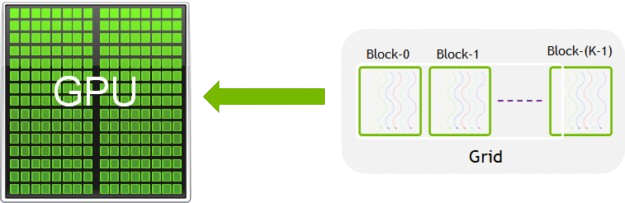
\includegraphics[width=\linewidth]{media/viz_blocks_grid.png}
        \caption{Visual representation of the CUDA hierarchy. \cite{Gupta_2023}}
        \label{cuda diagram}
    \end{figure}
    *Don't worry if you've never been exposed to C\texttt{++}, the syntax is essentially the same as C or Java, and you won't be doing anything too complicated. If your background is solely Python \href{https://web.stanford.edu/class/archive/cs/cs106b/cs106b.1252/resources/python_to_cpp.html}{here's a short guide with all the syntax you'll need}. Additionally, a small section on interfacing with pointers is included in the Colab.

    \newpage
    \textbf{Indexing Inside a Kernel}

    This hierarchy of \textbf{grid}, \textbf{block}, and \textbf{thread} forms the foundation of GPU programming, enabling organized parallel computations. But how can we use this for parallel processing?

    \vspace{10px}
    Every thread has a unique identifier, which can be determined by its position within its block, and the position of its block within the grid. By using these identifiers, threads can independently process data in a manner that corresponds to their specific task in parallel. The CUDA runtime provides these through the variables below, which are made available within any kernel that you write.

    \begin{itemize}
        \item \texttt{threadIdx.x}, \texttt{threadIdx.y}, \texttt{threadIdx.z}: A thread's index within its block in the x, y, and z dimension.
        \item \texttt{blockIdx.x}, \texttt{blockIdx.y}, \texttt{blockIdx.z}: A block's index within the grid along respective dimension.
        \item \texttt{blockDim.x}, \texttt{blockDim.y}, \texttt{blockDim.z}: \# total threads in each block along respective dimension.
        \item \texttt{gridDim.x}, \texttt{gridDim.y}, \texttt{gridDim.z}: \# blocks in grid across respective dimension. 
    \end{itemize}

    When launching a kernel with pyCUDA, we specify both the block size, \texttt{block}, and the grid size, \texttt{grid} we want to use to ensure we sufficiently cover the size of the input data. We will stick to a block size of $16 \times 16 \times 1$, and define our grid size based on the block size as and the size of the data.

    \vspace{10px}
    Using these variables, we can map locations in memory to physical hardware cores. As this problem will deal with 2D structures only, you'll only need to use the following lines of code.

    \begin{verbatim}
    int idx = threadIdx.x+blockDim.x*blockIdx.x;
    int idy = threadIdx.y+blockDim.y*blockIdx.y;\end{verbatim}
    There are of course, tons of additional systems-level and hardware-level details, but for this problem the only other detail you need to know is that GPUs have their global memory (VRAM), which is larger yet slower to access than the shared memory available to a given block.

    \vspace{10px}
    \textbf{General CUDA Workflow}

    Now, let's cover the typical framework to follow once you've established that a problem can be solved in parallel with a guided example. Create a copy of the Google Colab environment for this project \href{https://colab.research.google.com/drive/1Y38N7kXJuTd-TPAA5fzQLVsc25rI9Qkc?usp=sharing}{linked here} and follow along until you reach the next section.

    \newpage
    \textbf{Matrix Multiplication Kernel}
    
    Now, it's your turn to dive deeper.
    \vspace{10px}
    
    Matrix operations are a necessity at every step of training a deep learning model, from data augmentation to neuron activations and backpropagation. By definition, linear operators are distributive, and thus most of the matrix operations used behind the scenes of deep learning are known as \textit{embarrasingly parallel} problems, since individual operations can be computed independently and brought together after.

    \vspace{10px}

    Your task is to implement a kernel to compute the matrix multiplication 
    \begin{gather*}
        C = AB \\
        dim(A) = n \times m \\
        dim(B) = m \times p
    \end{gather*}
    
    \vspace{10px}
    
    Hint, recall the dot product definition of matrix multiplication
    \[
        C_{ij} = \sum_{k=1}^{m} A_{ik} \cdot B_{kj}
    \]

    \vspace{10px}
    \textbf{Tasks}
    \begin{enumerate}
        \item Include a shareable link to your Colab. \hfill (required)
        \item Write down how long it takes for your \texttt{doublify} kernel to execute for $n=2^{12}$. \hfill (2 pts)
        \item Copy the benchmarks graph you made for your \texttt{matmul} kernel, and describe the runtime trends you see. \hfill (10 pts)
        \item Explain (don't implement) 2 nontrivial* ways your \texttt{matmul} kernel could be optimized for speed. This can be either software or hardware-dependent. \hfill (3 pts)

    \end{enumerate}

    If you liked this problem, consider reading through \href{http://courses.cms.caltech.edu/cs179/}{CS179}'s course materials.
    
    
\end{problem}


\begin{solution*}{}{}
\begin{enumerate}
    \item \href{https://colab.research.google.com/drive/10ih_KraR17stg4llNfxWk82pU-lto32N?usp=sharing}{colab link}
\item Kernel Speed: 0.000663 seconds
\item The runtime grows exponentially with matrix size for both methods, and the
    gpu runs twice as fast for large matrix sizes (8192 and 16384).
\begin{center}

\includegraphics[width=0.8\textwidth]{media/5.png}
\end{center}
\item To make it faster, we can store $B$ as $B^{T}$ instead the GPU caches rows
    of values together as they are closer together in the 1D flattened array,
    and thus are likely to be cached together when accessed (I know this is true
    for CPUs at least from CS 24). We can also load the memory for the
    corresponding blocks into the shared memory so there's no transfer speed
    delay and use TPUs.
\end{enumerate}
\end{solution*}

\newpage{}
\begin{problem}{Representation power \hfill[20 pts]}{prob:rep_power}

\begin{enumerate}
\item Show that adding layers to a neural network without non-linear activation functions does not increase its expressive power. \hfill (4 pts)
\item Give an example where adding layers to a deep network without non-linearities could reduce the expressive capacity of the network. \hfill (3 pts)
\item Design a one-layer perceptron that fits the logical functions \texttt{AND} and \texttt{OR} for 2D inputs. Why can't a single layer fit \texttt{XOR}? \hfill (5 pts)

\item Show that a neural network with a one-dimensional input $x$ and one-dimensional output $y$, with ReLU activations of depth $D$ and widths $W_d$, $d=1,\dots,D$ can represent piecewise linear functions $f$ with at most $2^D \prod_{d=1}^{D} W_d$ linear pieces.

Essentially, if we define $\kappa(f)$ as the smallest number of linear pieces in $f$, show
\[
\kappa(y) \le 2^D \prod_{d=1}^{D} W_d
\]

Here are some hints.
    \begin{enumerate}[a.]
        \item We can always represent a piecewise linear function with $N$ pieces as a one-layer network with width $N$ (case $D=1$)
        \item Proceed by induction, keeping in mind that
        \begin{enumerate}[i.]
            \item The property is invariant to scale (the number of linear pieces of $f$, $\ell_f$ needs remains the same regardless of scaling $f$)
            \item The number of linear pieces in the sum of two functions is at most the sum of the number of linear pieces in each individual function.
            \item Applying a ReLU to a function at most doubles the number of linear pieces needed
        \end{enumerate}
    \end{enumerate}

\end{enumerate} 

It might help you to draw out piecewise functions for problem 4. \hfill (8 pts)
\end{problem}

\begin{solution*}{}{}
\begin{enumerate}
\item \begin{proof}
Every layer in a neural net is a linear map. Thus, if there are no activation
functions, the network is a composition of linear maps, which we know is another
linear map, which is not an increase in expressive power.
\end{proof}

\item Say you have an input layer of size $d > 1$ and an initial final layer of
size $d$. If you add an intermediate layer of size $1$, you reduce the
expressive capacity since you go from a higher dimensional space to a latent
space between the first and second layers, and then go from a latent space to a
space that has the same dimensions as the initial space, which we know can no
longer be spanned by the inputs of the previous layer. 

More formally, let our target function be a linear map $f:\mathbb{R}^{d} \to
\mathbb{R}^{d}$. A single layer neural network without activation can
theoretically learn this since the network itself is a linear map
$g:\mathbb{R}^{d} \to \mathbb{R}^{d}$. However, if we introduce an intermediate
layer with dimension $c < d$, then we first go from $\mathbb{R}^{d}\to
\mathbb{R}^{c}$, and then go from $\mathbb{R}^{c}\to \mathbb{R}^{d}$ for the
output. However, $\mathbb{R}^{c}$ doesn't span $\mathbb{R}^{d}$, so the output
cannot span $\mathbb{R}^{d}$ either.

\item A perceptron with the weights $(1, 1)$ and bias $-1.5$ could simulate AND,
    and a perceptron with weights $(1, 1)$ and activation threshold $-0.5$ could
    simulate OR, where negative output means false and positive means true. We
    can't simulate XOR with a singe layer since a single layer is a line, and
    XOR is not linearly separable (can't be separated by a single line).

\item \begin{proof}
Each neuron with a ReLU activation is able to split each of its inputs into a
piecewise linear function consisting of two parts: if $x_{i}$ is the input value
and $w_{i}, b_{i}$ are the weight and bias corresponding to that input for the
neuron, the ReLU activation creates a flat line for $w_{i}x_{i} + b_{i} < 0$ and 
another line of slope 1 for $w_{i}x_{i}+b_{i} \ge 0$. 

Now, consider every single path that can be taken from an input value through
the network. There are $W_{1}$ neurons to choose from in the first layer, $W_2$
neurons to choose from in the second layer, and so on for each of the $D$
layers. And at each of the $D$ steps/neurons in the path, the ReLU activation
function can double the number of linear pieces within the function
corresponding to the path that's been taken. We know that the number of linear
pieces in the sum of two functions is at most the sum of the number of linear
pieces in each individual function, since this happens when none of the
intervals for each piece in either function share an endpoint with an interval
for a piece in the other function. Thus, the the maximum number of pieces of the
neural network is the sum of the number of linear pieces created by all the
functions corresponding to the paths that could have been taken from the input
to the end of the network, which is

\[
2^{D}\prod_{d=1}^{D} W_{d} 
\] 

since at each of the $D$ steps, we can create 2 new pieces, and the are
$\prod_{d=1}^{D} W_{d}$ neurons to choose from at each layer/step when going
forward through the network.
\end{proof}
\end{enumerate}
\end{solution*}

\newpage

\vfill

\bibliographystyle{unsrtnat}
\bibliography{references}

\end{document}
